\section{Introduction}\label{sec:intro}

Today's file systems provide two primary functions: a way to store chunks of data and names that provide users with the familiar
metaphor of a file cabinet (i.e., folders and documents).
Much has changed since we adopted this design. 
Now most data does not reside on local file systems because instead data is distributed across myriad services such as Dropbox, Google docs, Amazon S3, Microsoft OneDrive, and Github as well as attached to communication mechanisms and applications like email, chat, and Slack.
Today, just like local file systems, each of these storage solutions provides its own storage and naming mechanisms.
And therein lies the problem: names were and are designed for users, but multiple disparate namespaces hurt the user experience.
The user bears the burden of remembering personally irrelevant information: \textit{where} they stored their documents.
In the worst case, they must search through the individual storage silos. There is no practical/convenient way to quickly locate the item.

Existing solutions tie namespaces to storage silos, but this model does not fit with the way we use storage.  
We routinely access data from multiple silos, locating items by navigating or searching silo-by-silo.

We observe that names serve two purposes: names specify \textit{location} and/or \textit{context or semantic meaning} of the object.  
Context/meeting is most important to users; location is most important to the storage silo.
Typically, storage systems fuse these naming purposes in such a way that it is not possible to relegate
fixing the context/semantic naming problem to the Human Computer Interface (HCI) community.

The following (real world) scenario highlights some of the challenges.

A student from the country of Lemuria is destined for a summer internship in Camelot. Arranging for this internship
requires many (many, many) different data objects: email messages with the host, offer letters, academic forms, a visa, 
boarding passes, project proposals, and more. How can our overwhelmed intern organize and/or find all the documents 
associated with their internship? We consider three approaches.

\textit{Meticulous:} Place/copy every document into a single directory on their personal machine. 
Pros: It is simple to find everything. 
Cons: It requires conscious effort, pre-planning, and prescience.  Everything is saved: emails,
copies of physical documents, text messages, and project proposals. Our intern hopes they have correctly predicted what they will
need in future.  With more files and people involved, record keeping takes more time and people have different opinions on how to organize the files.

%When the student begins the process by sending tens of email messages, must they all be exported from mail and saved away? 
%Each time the shared project proposal changes, the student must update their local copy. 
%Further, this approach does not scale because as the number of files and people involved increases, the complexity increases
%exponentially, which becomes untenable.

\textit{Haphazard:} Leave everything where it is and search for it when you need it. 
Desktop search utilities such as Spotlight~\cite{apple-search} and application-specific search tools make this possible, 
but this approach frequently requires searching across multiple silos, returns many more documents than intended, and misses those our intern~\cite{bergman2019factors}.

\textit{Nirvana:} Our tool on the intern's local machine creates a \textit{personal namespace}. 
It combines conventional file system metadata with new (optional) user-provided metadata, relationships between items (e.g., an email
message and the document attached to it, email messages with largely identical contents, and documents shared among the same sets of people)
and provides a navigation interface that uses this metadata to create collections of semantically related objects~\cite{gifford1991semantic}.

We tried to implement Nirvana outside the storage system~\cite{ashish}. 
We developed a visualizer that constructed personal namespaces by extracting existing and new properties (primarily relationships similar to those listed above) from multiple distinct data storage silos.  
We were surprised at the effectiveness of this approach to find related files, even across storage silos, particularly when combined with additional metadata that we generated. 
%Figure \ref{fig:ashish-demo} shows a screen capture from a demonstration of that visualizer. 
%\mis{I find this particular visualization confusing; is it possible to create the one where all the documents just magically showed up? The relationships here dominate and don't necessarily make sense in this context.}

%Based on this experience, we concluded that dynamically generated, per-user namespaces are a promising solution to today's multi-silo reality, but that the promise of such systems cannot be realized without storage system support and integration. 
%\mis{do better than this: The rest of this paper explores exactly what kind of system support is required.}

Building Nirvana within the confines of existing storage silos has limitations:
(1) using static file system attributes hindered us from providing useful ways to search and navigate data, 
(2) extracting file relationships across storage silos without explicit support for relationships as \textit{attributes} was tedious, 
(3) our visualizer had no mechanism of maintaining privacy and security when storing these attributes outside the storage silos. 
Our observation is that dynamically generated, per-user namespaces show promise when used with today's multi-silo reality. 
However, this promise cannot be realized without storage system support and integration.
We propose the Nirvana architecture, which separates \textit{location names} from \textit{context/semantic names}, and provides 
the latter \textit{outside} of the storage system via a separate namespace service.

The idea of having distinct namespace providers delivering a global namespace is not new~\cite{howard1988scale,kazar1990decorum}, 
nor is the idea of using file metadata to generate namespaces ~\cite{gifford1991semantic}.
Nirvana is novel in that it combines these pre-existing ideas, introduces new approaches, and is specifically designed to support today's multi-silo world.
Nirvana combines 1) support for multiple namespace providers, 
2) an expansive view of storage meta-data, 
3) embracing search as an essential component of naming, and 
4) a separation of user-visible names from silo-local names.

The rest of this paper introduces Nirvana and explores what system support is required to realize this vision.

%In the next section, we highlight prior work that either addresses similar issues or presents building blocks upon which a solution might be developed.
%Then, we propose a an architecture for the construction and maintenance of personal, multi-silo namespaces.
%Based on this proposed architecture, we then identify and discuss the research challenges that must be addressed to realize such a vision.

%\begin{figure*}
%    \centering
%    \begin{tabular}{ccc}
%        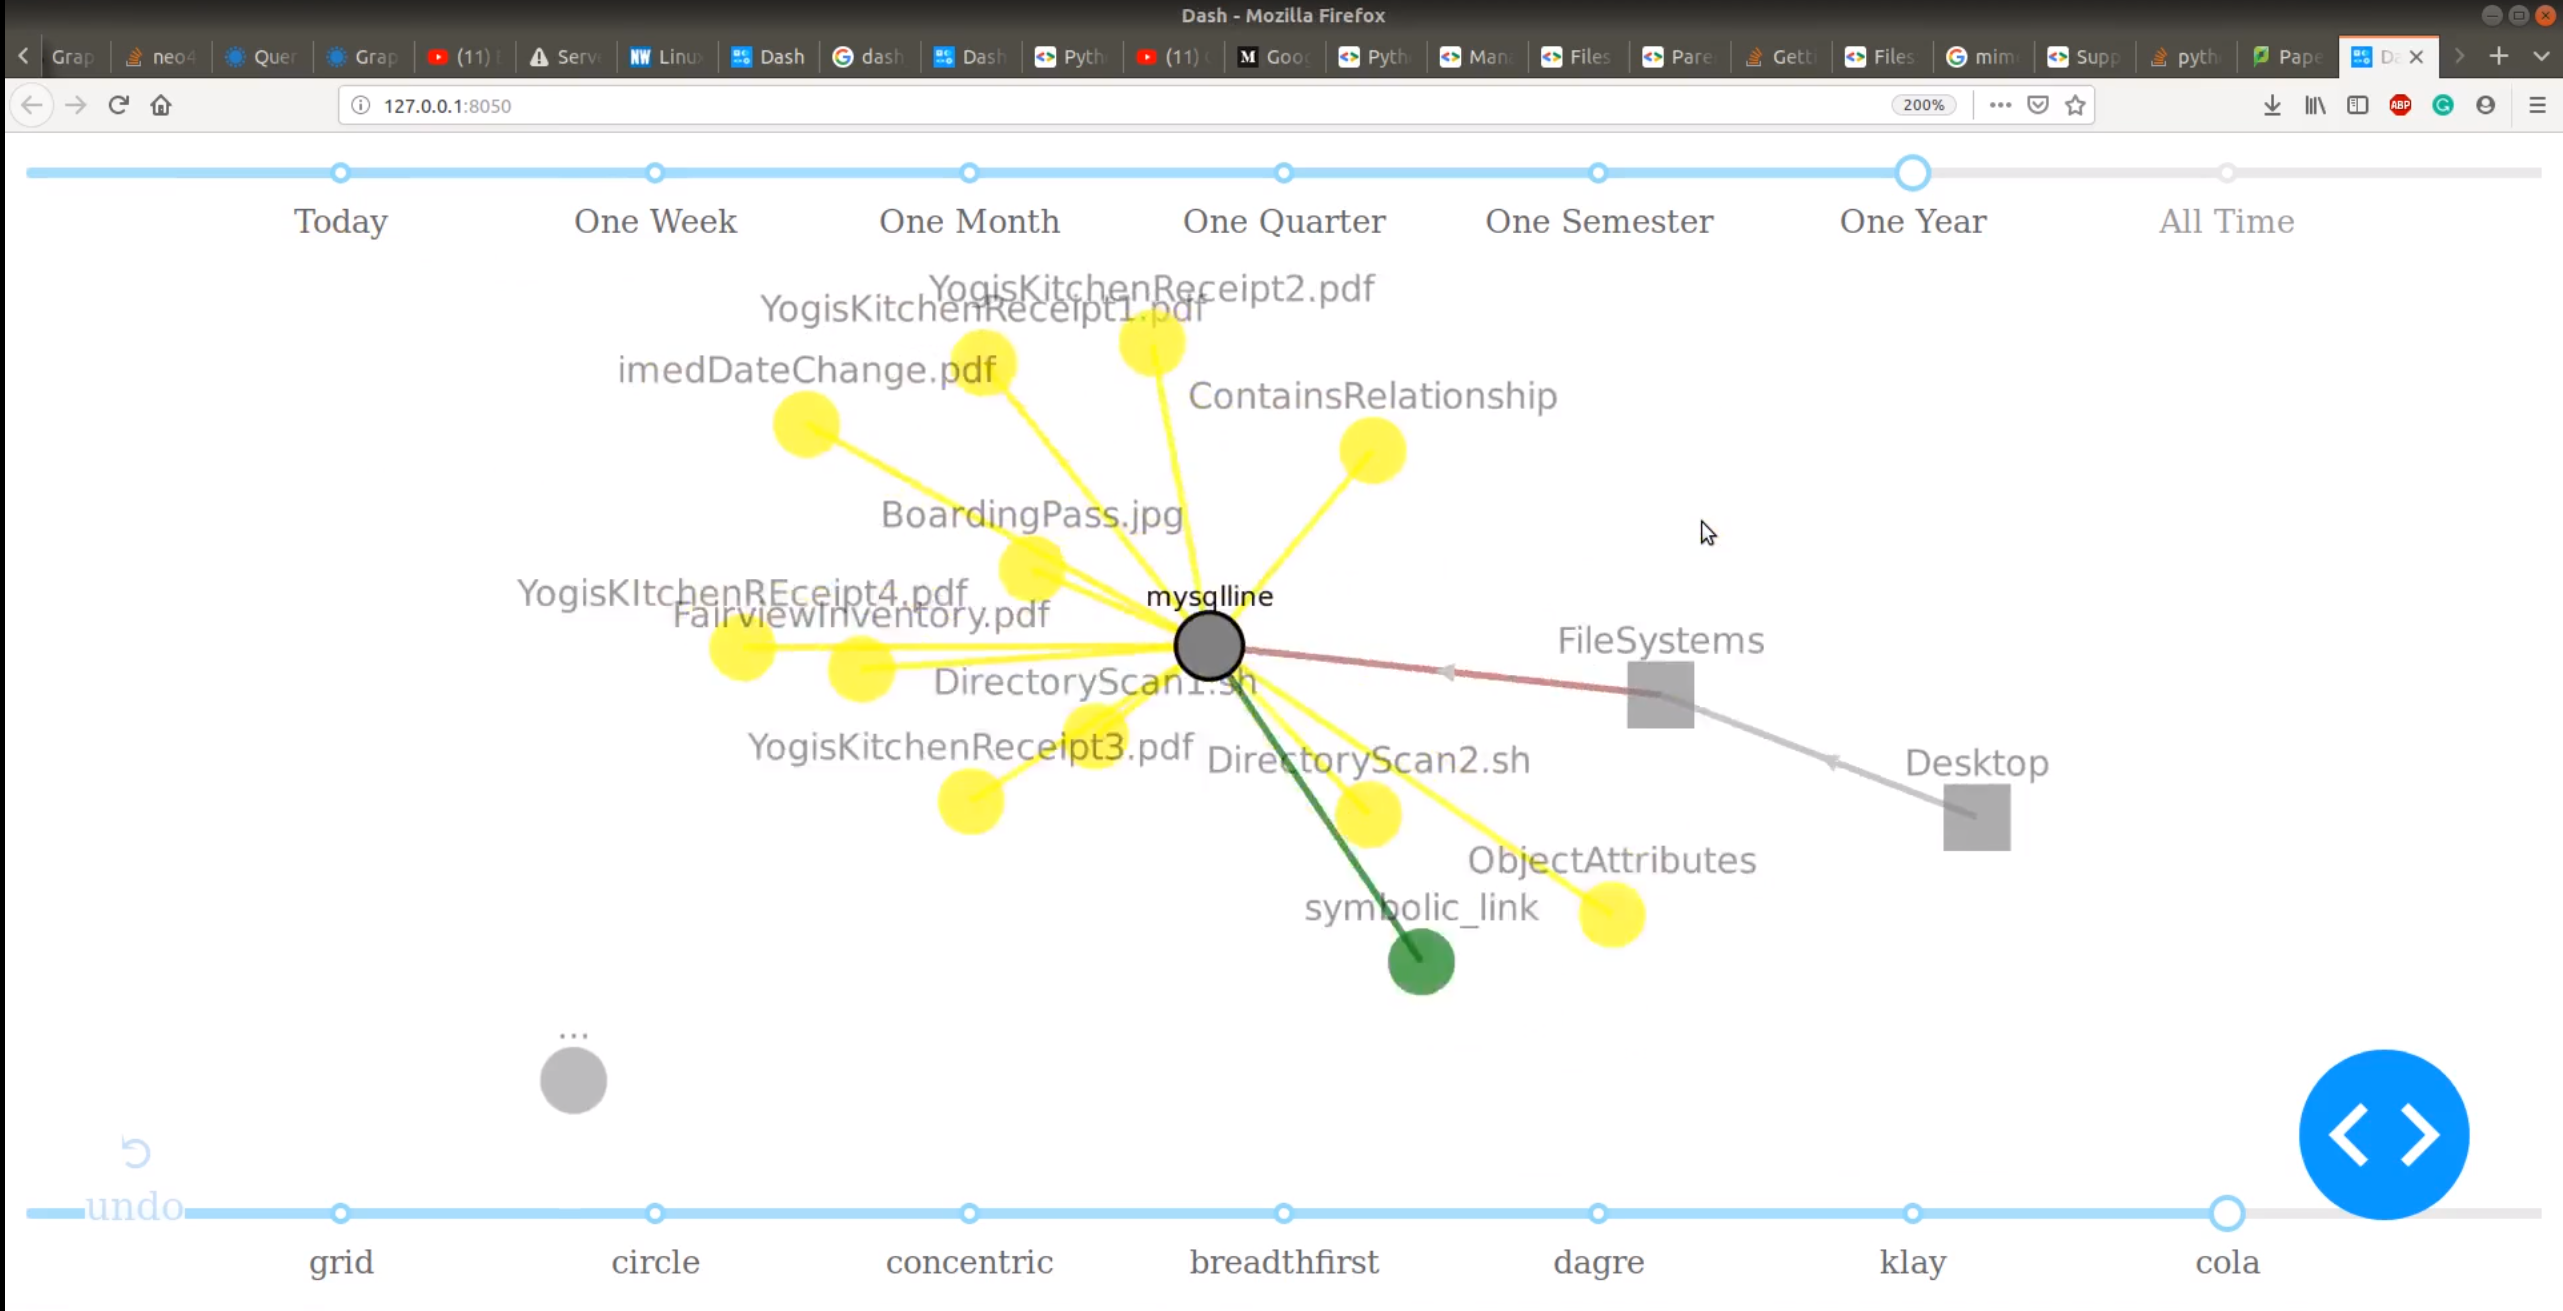
\includegraphics[width=0.3\textwidth]{figures/ashis-graph-data-visualizer-demo-screenshot.png}
%        &
%        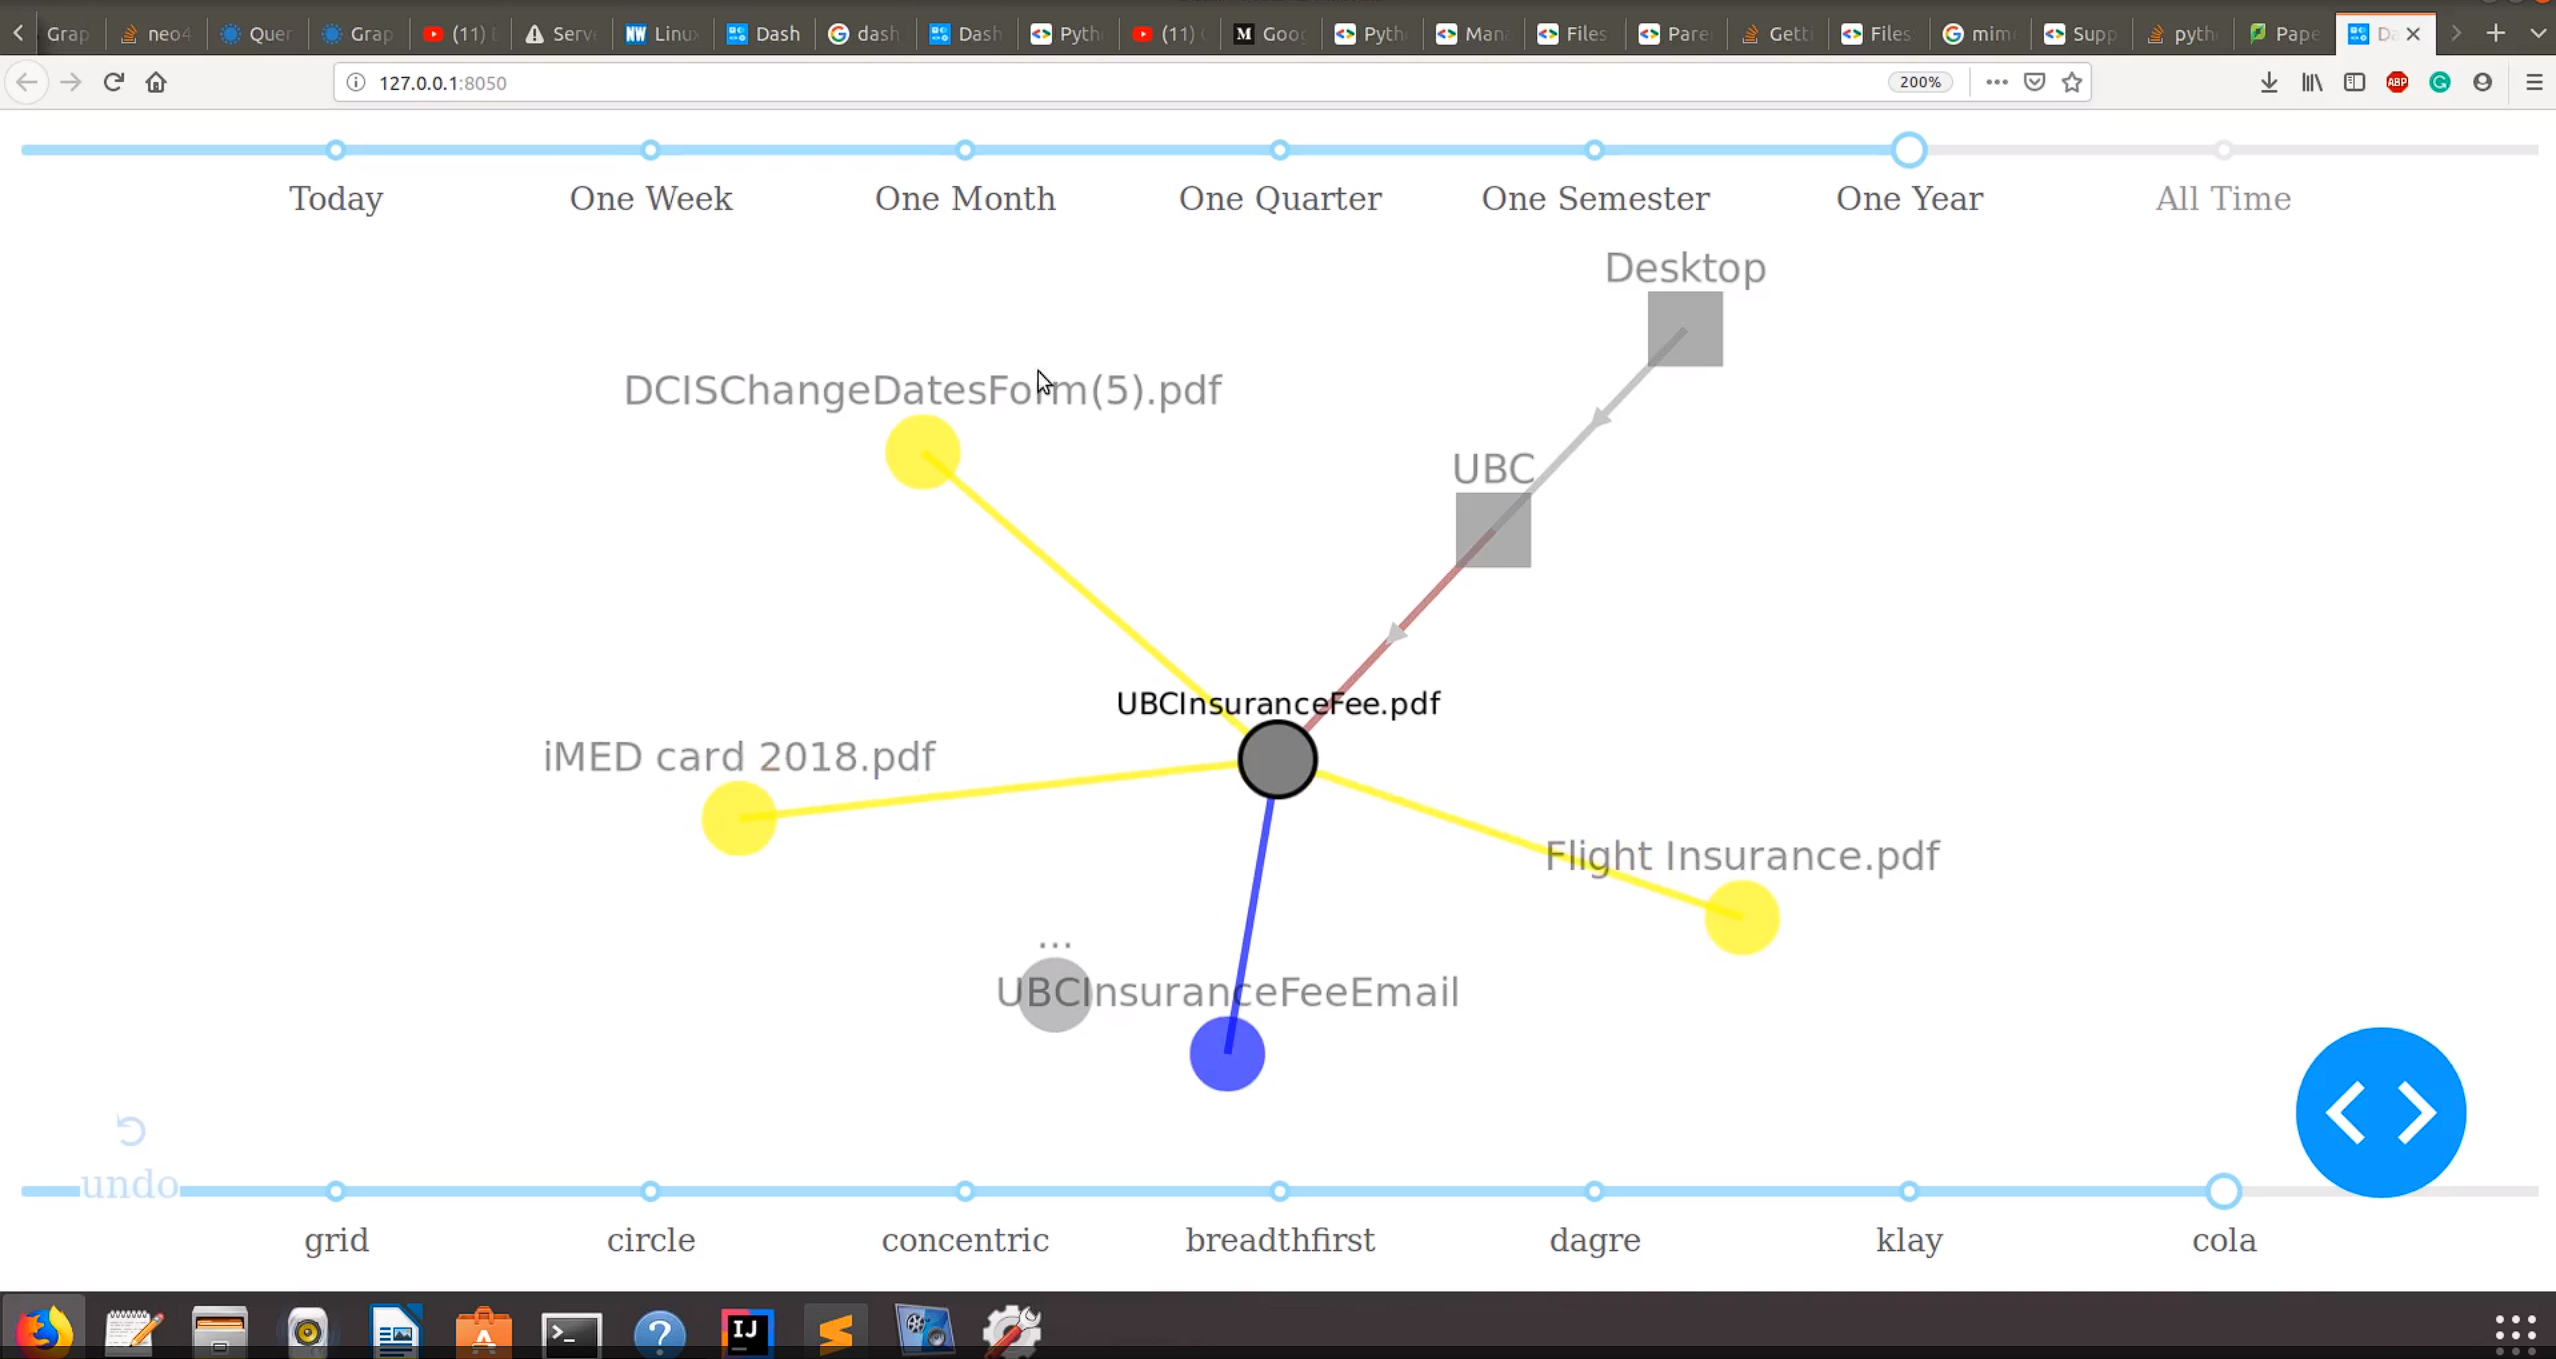
\includegraphics[width=0.3\textwidth]{figures/ashish-graph-data-visualizer-demo-1.png}
%        &
%        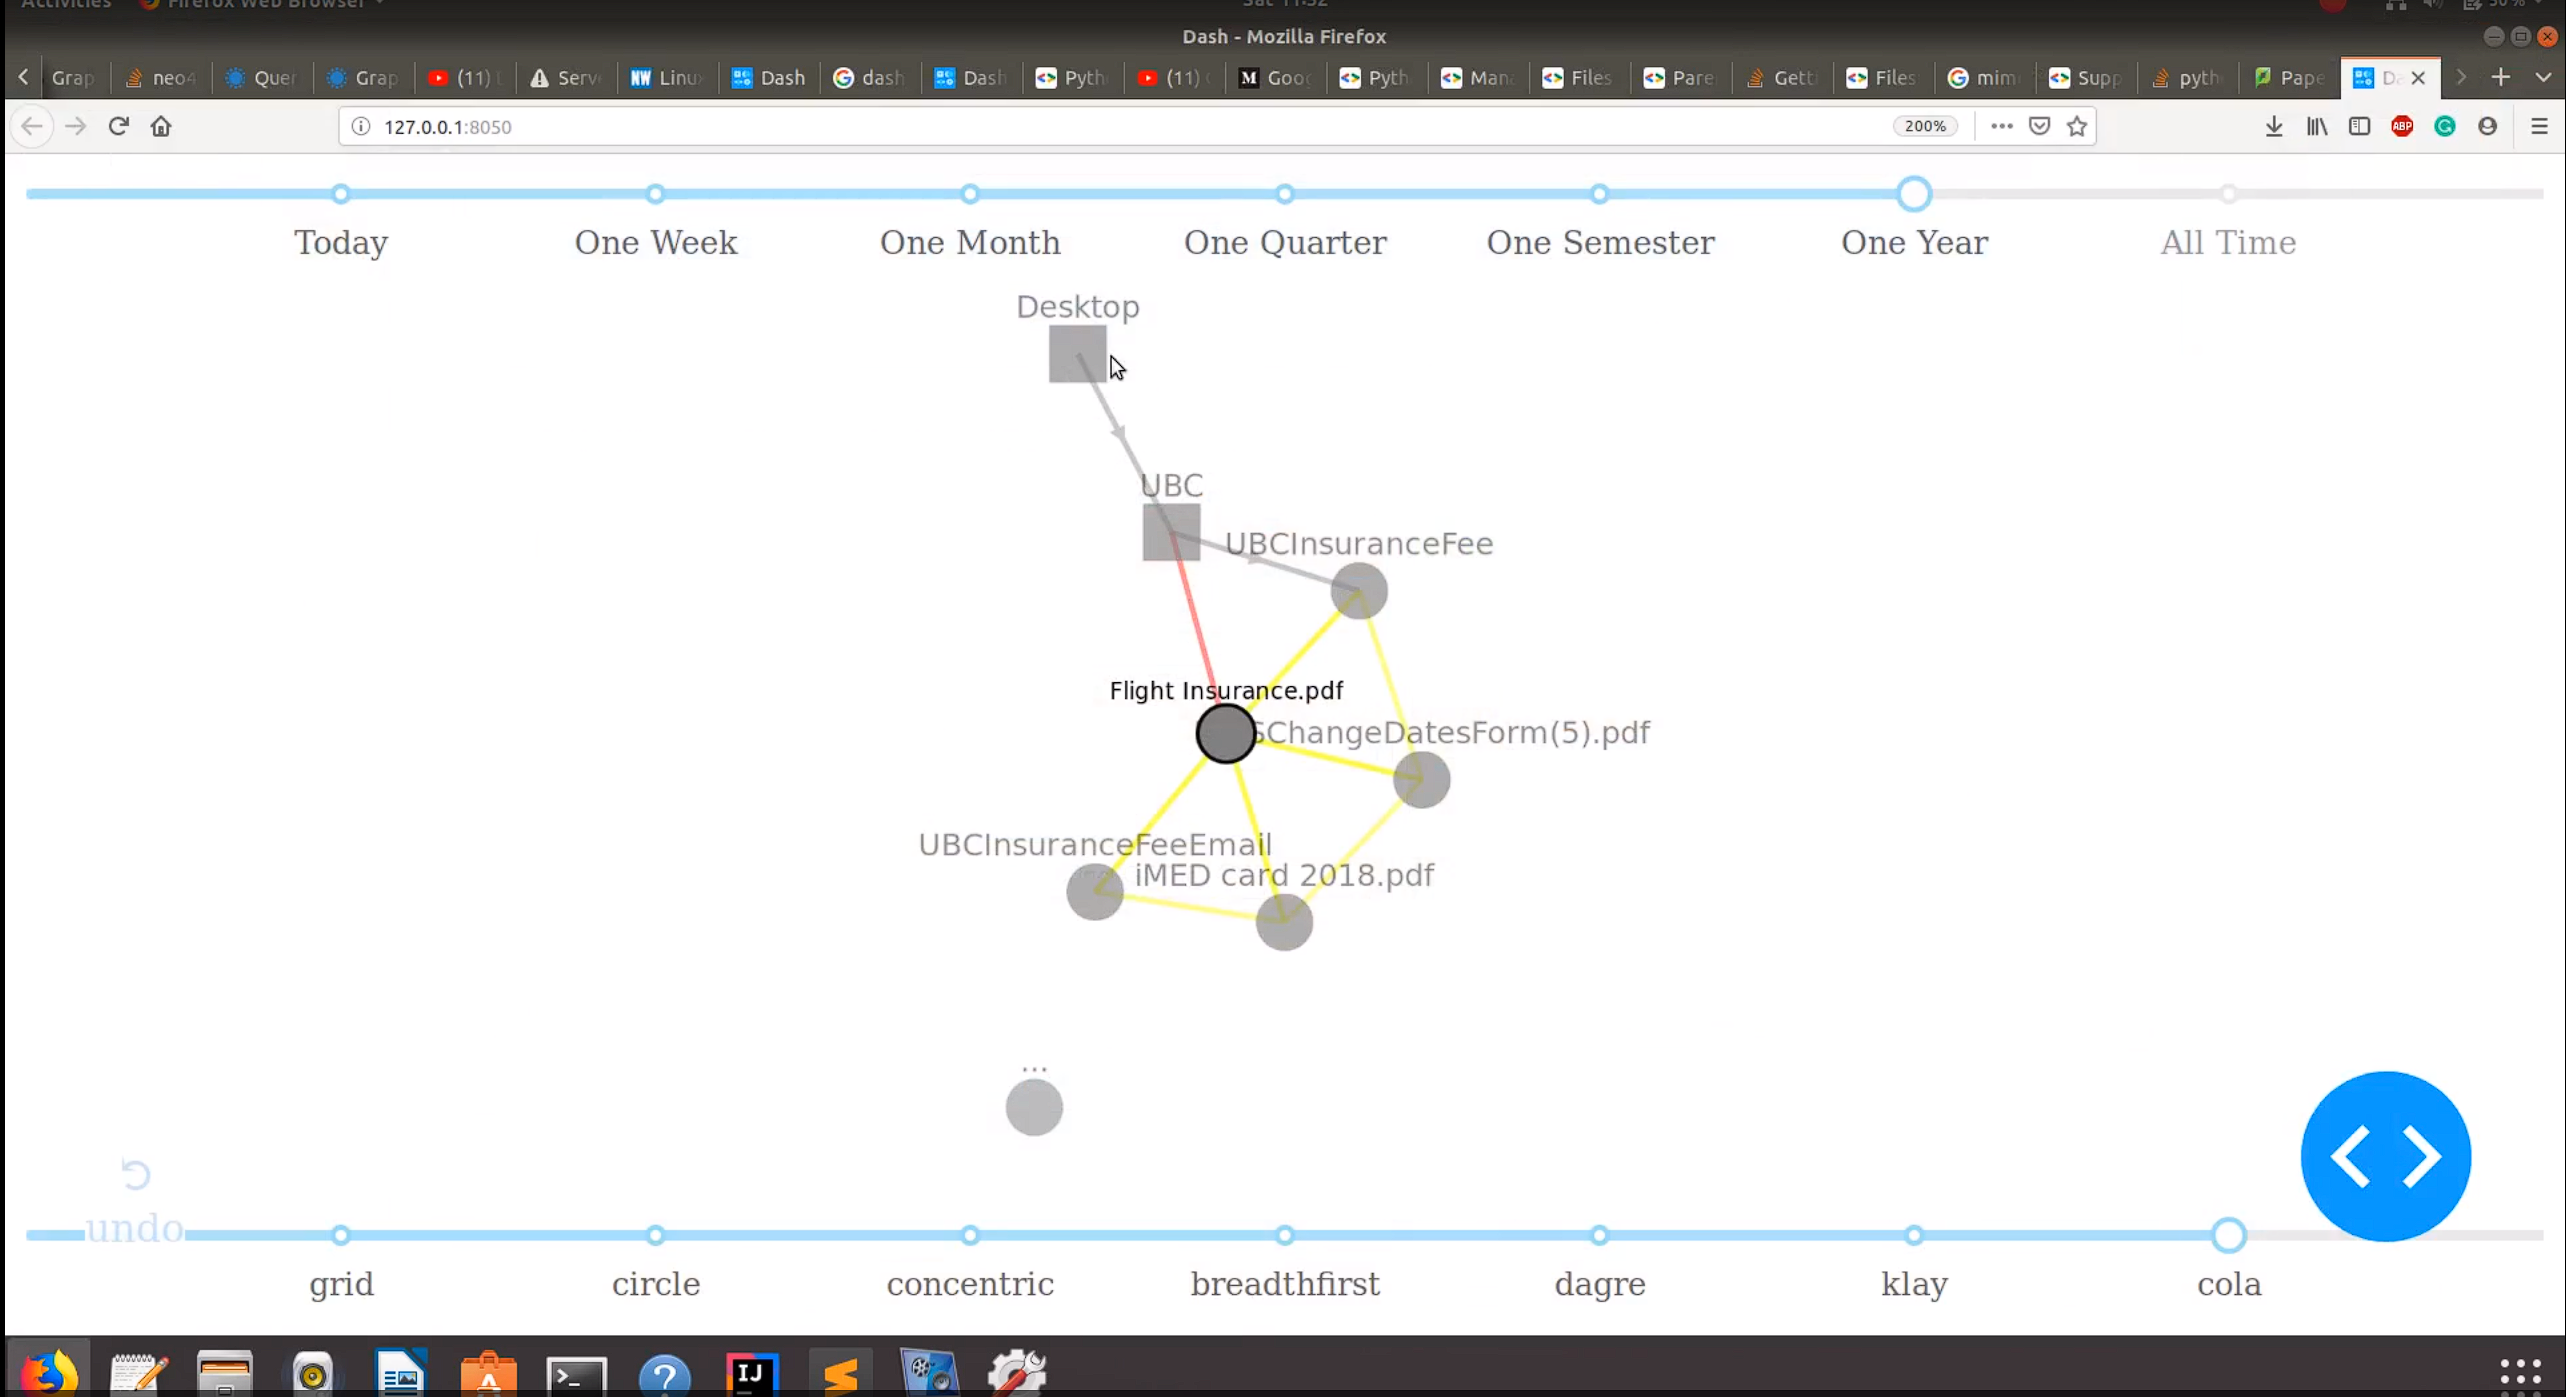
\includegraphics[width=0.3\textwidth]{figures/ashish-graph-data-visualizer-demo-2.png}
%        \tabularnewline
%        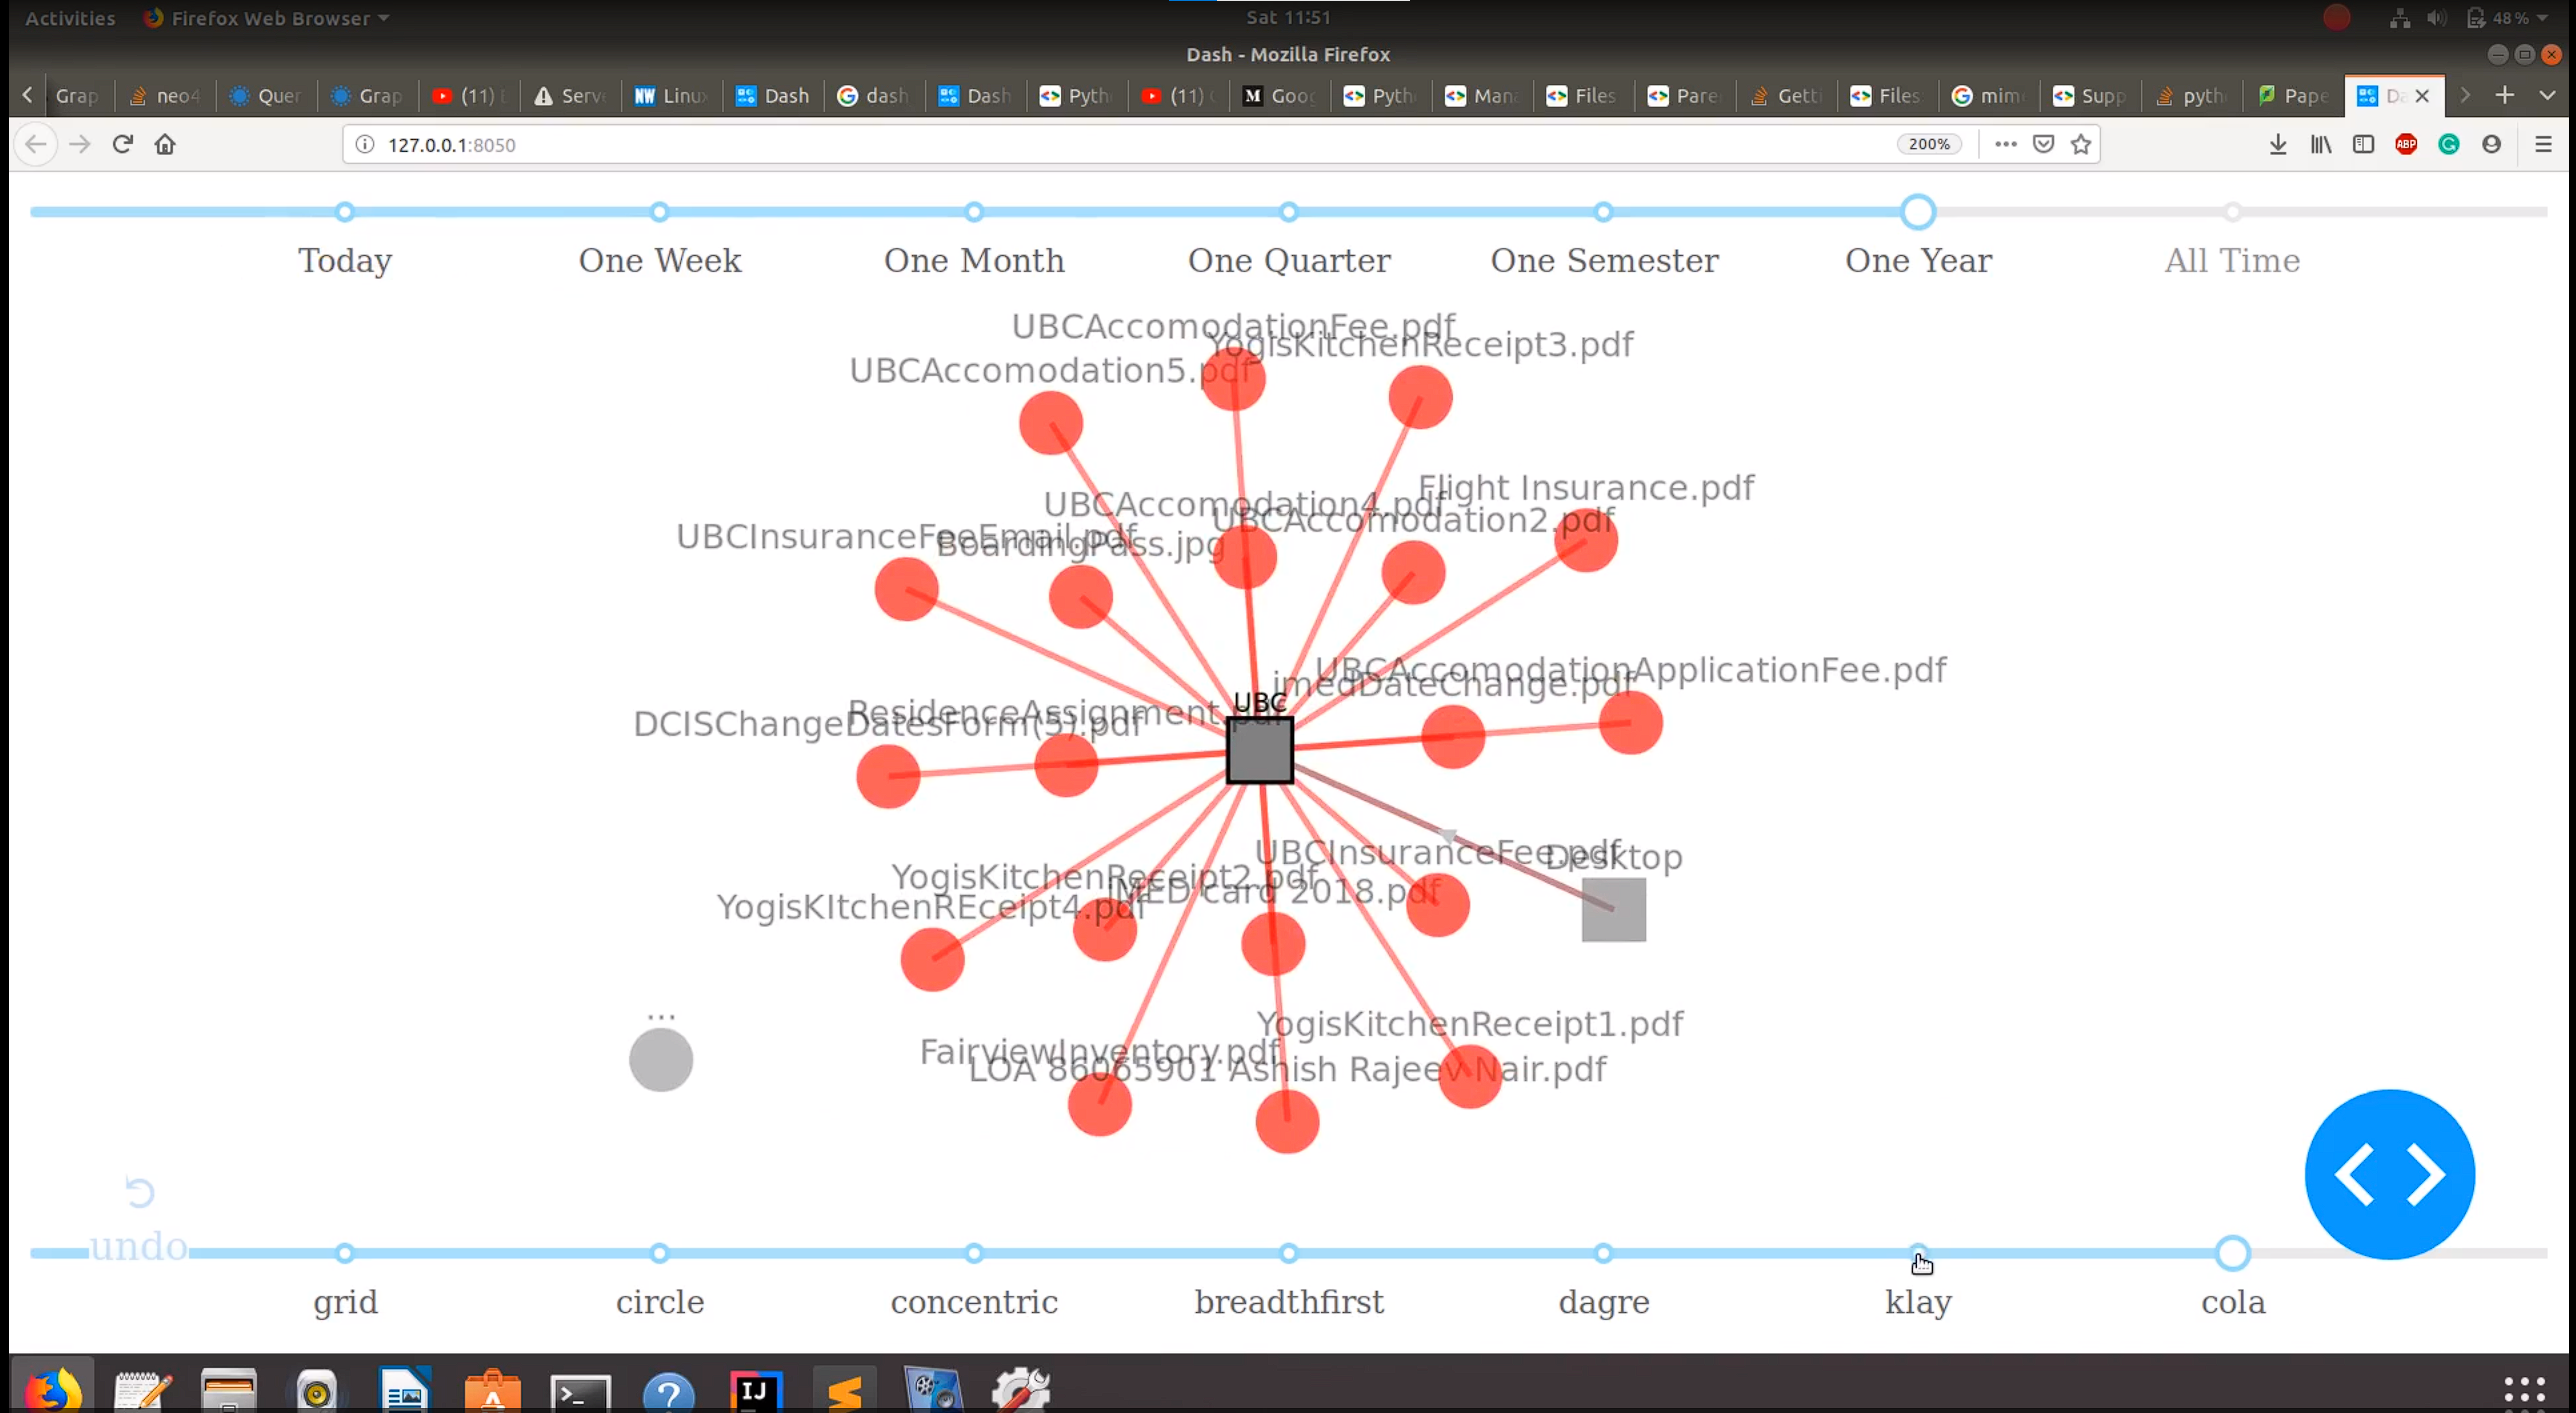
\includegraphics[width=0.3\textwidth]{figures/ashish-graph-data-visualizer-demo-3.png}
%        &
%        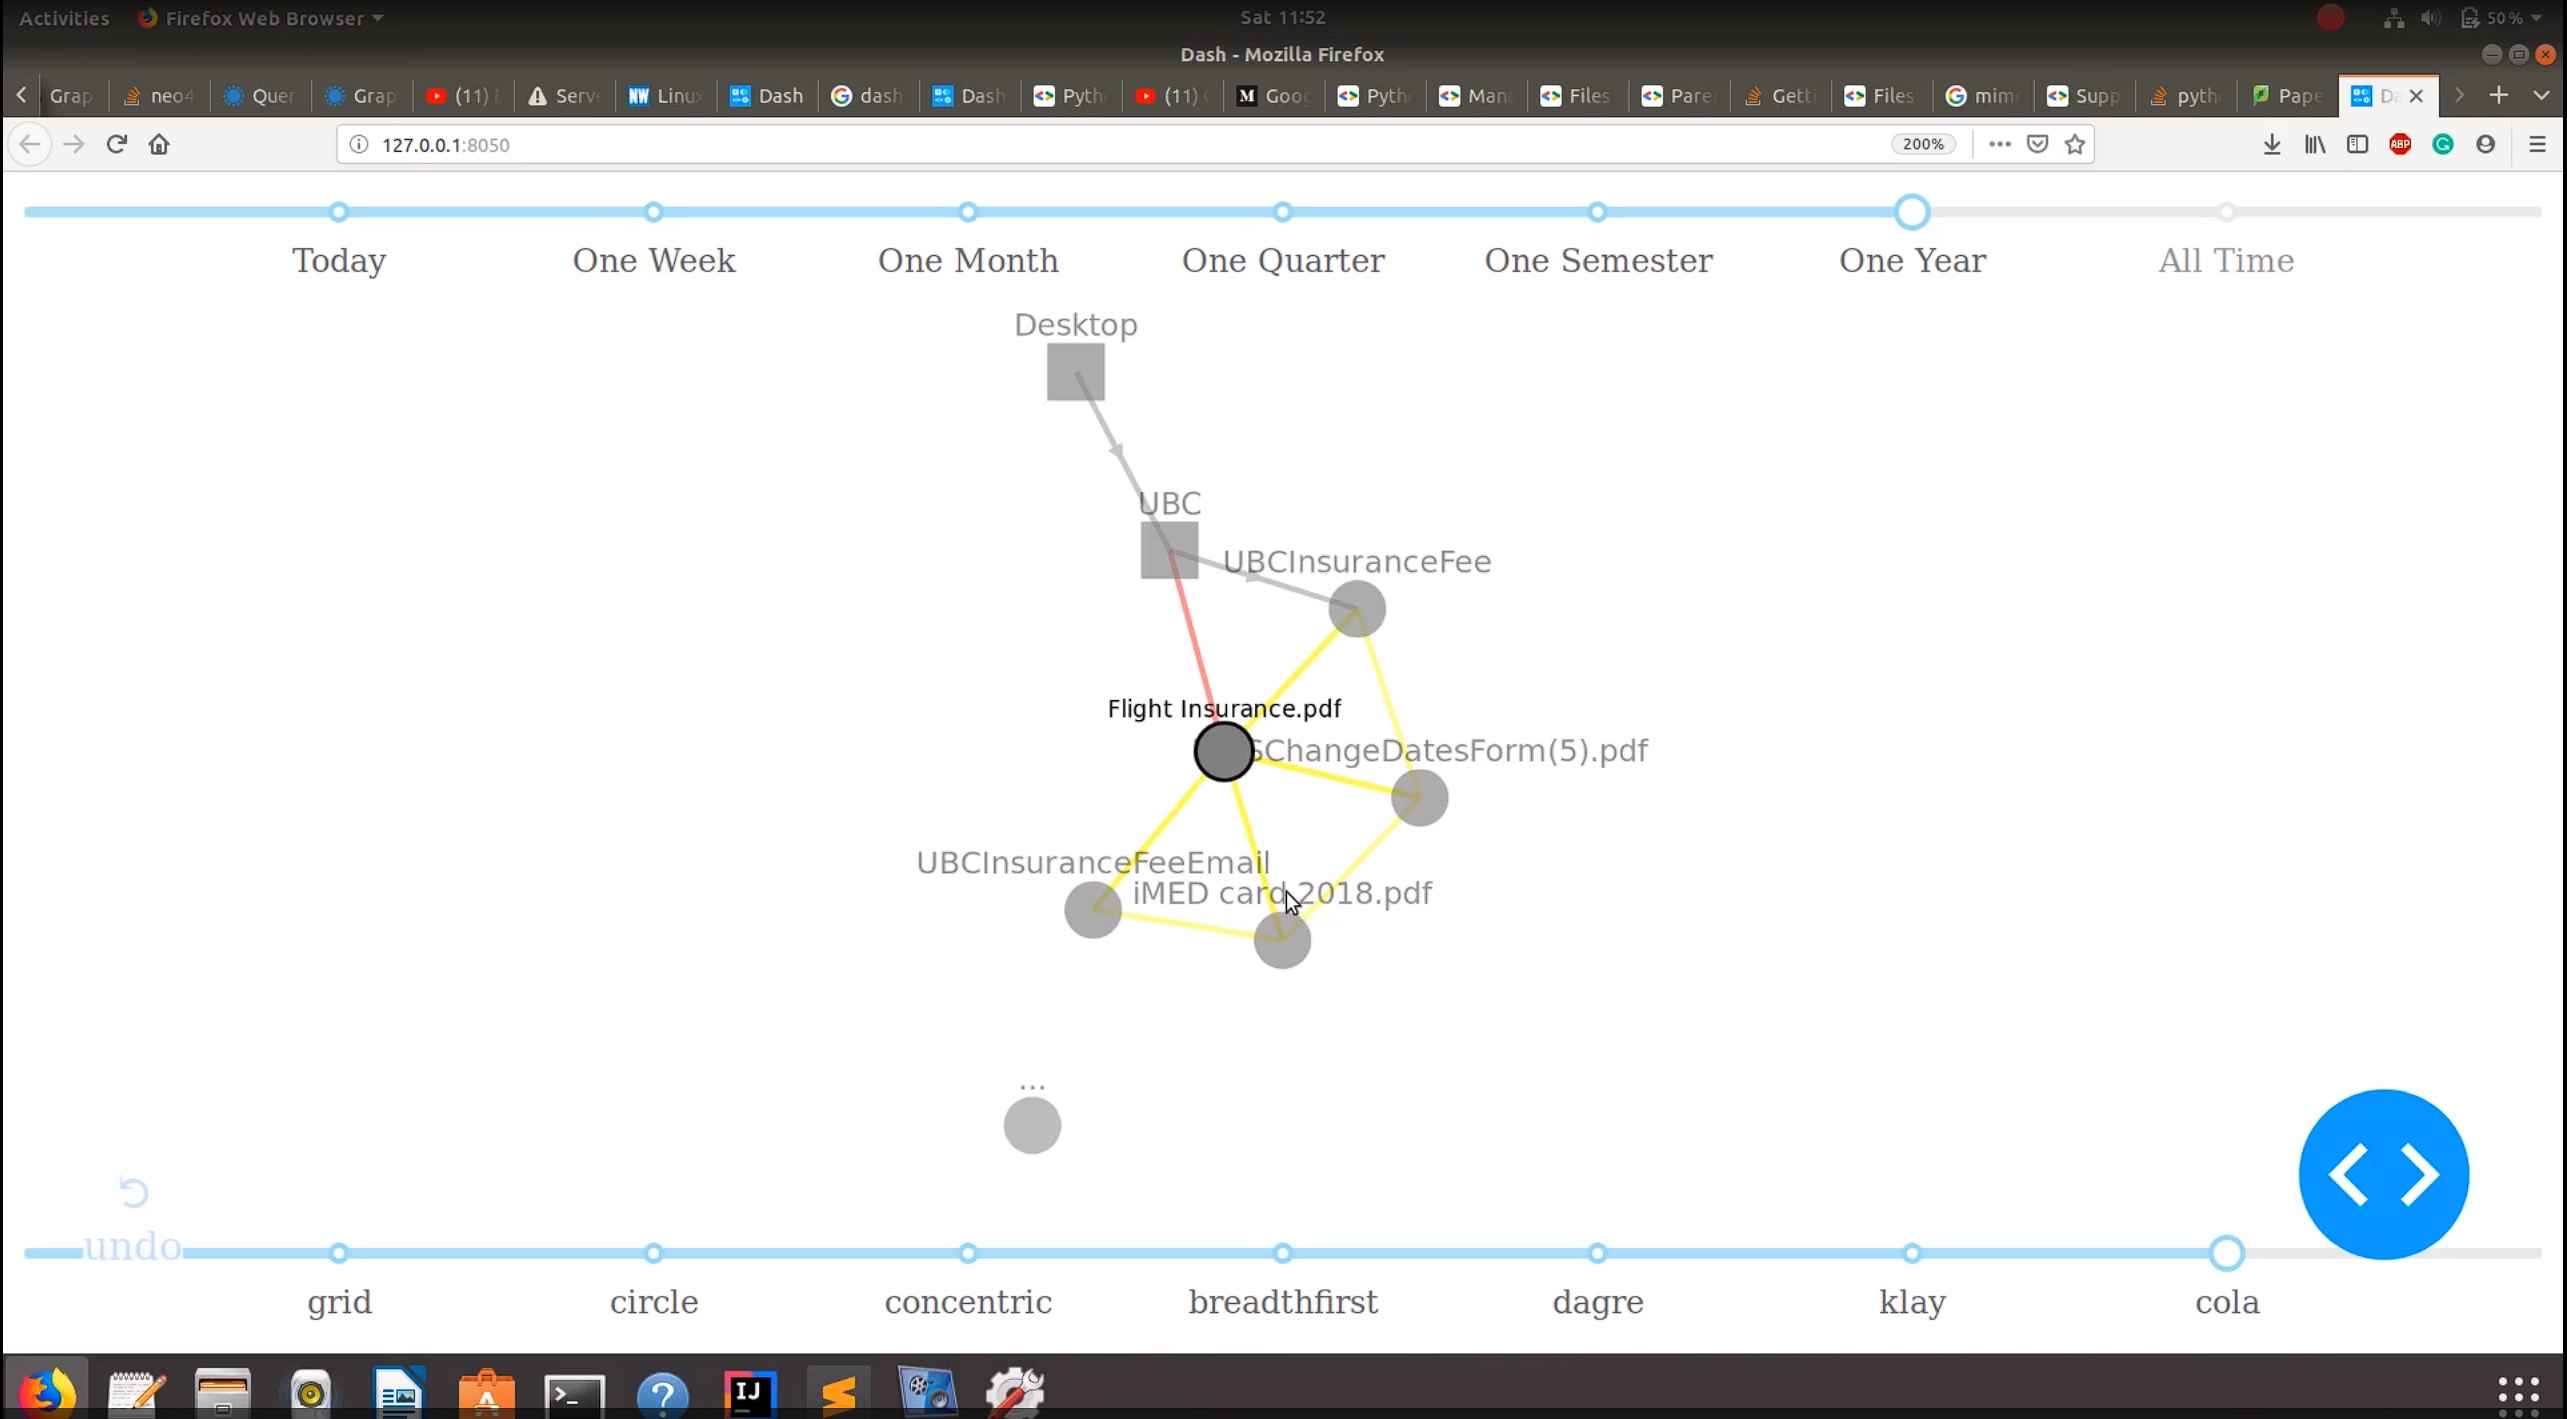
\includegraphics[width=0.3\textwidth]{figures/ashish-graph-data-visualizer-demo-4.png}
%        &
%    \end{tabular}
%    \caption{Pick One (or reject them all and find something else from Ashish demo that works).\\Then we need to sanitize the image.}
%    \label{fig:ashish-demo}
%\end{figure*}







